\part{Complex-Valued-Roots}
\lecture{Complex Valued Roots}{Complex-Valued-Roots}
\section{Ordinary Differential Equations}

\title{Ordinary Differential Equations}
\subtitle{Math 232 - Complex Values Roots}
\date{27 September 2013}

\begin{frame}
  \titlepage
\end{frame}

\begin{frame}
  \frametitle{Outline}
  \tableofcontents[currentsection]
\end{frame}


\subsection{Second Order, Homogeneous, Constant Coeff DEs}

\iftoggle{clicker}{%
\begin{frame}
  \frametitle{Clicker Quiz}

      \ifnum\value{clickerQuiz}=1{%

        \vfill

        Determine the roots to the characteristic equation associated with the DE
        \begin{eqnarray*}
          y'' + y' + y & = & 0.
        \end{eqnarray*}

        \vfill

        \begin{tabular}{ll}
          A: & $-\half\pm\frac{\sqrt{-3}}{2}i$ \\  [12pt]
          B: & $-\half\pm\frac{\sqrt{3}}{2}i$ \\  [12pt]
          C: & $1,-1$ \\  [12pt]
          D: & $-1\pm\frac{\sqrt{3}}{2}$
        \end{tabular}

        \vfill

      }\fi

      \ifnum\value{clickerQuiz}=2{%

        \vfill
        Determine the roots to the characteristic equation associated with the DE
        \begin{eqnarray*}
          2y'' + y' + 3y & = & 0.
        \end{eqnarray*}

        \vfill

        \begin{tabular}{ll}
          A: & $-\half\pm\frac{\sqrt{23}}{2}i$ \\ [12pt]
          B: & $-\half\pm\frac{\sqrt{23}}{2}$ \\  [12pt]
          C: & $-\frac{1}{4}\pm\frac{\sqrt{23}}{4}i$ \\  [12pt]
          D: & $-\frac{1}{4}\pm\frac{\sqrt{-23}}{4}i$
        \end{tabular}


        \vfill

     }\fi

     \ifnum\value{clickerQuiz}=3{%
      Determine the roots to the characteristic equation associated with the DE
        \begin{eqnarray*}
          y'' + y' + y & = & 0.
        \end{eqnarray*}

        \vfill

        \begin{tabular}{ll}
          A: & $-1\pm\sqrt{-3}i$ \\ [12pt]
          B: & $-1\pm\sqrt{-3}$ \\  [12pt]
          C: & $-\frac{1}{2}\pm\frac{\sqrt{3}}{2}$ \\  [12pt]
          D: & $-\frac{1}{2}\pm\frac{\sqrt{3}}{2}i$
        \end{tabular}

        \vfill

    }\fi


\end{frame}
}


\begin{frame}
  \frametitle{Formulas}
Formula 1:
  {\color{brown}
  \begin{eqnarray*}
  \sqrt{-3} & = & i\sqrt{3}\\
  \sqrt{-c} & = & i\sqrt{c}, c \text{ is a positive number}
  \end{eqnarray*}
  }

Formula 2:
  {\color{red}
  \begin{eqnarray*}
  e^{a+bi} & = & e^a (\cos(b) + i\sin(b))\\
  e^{a-bi} & = & e^a (\cos(b) - i\sin(b))\\
  \end{eqnarray*}
  }

Formula 3:
  {\color{blue}
  \begin{eqnarray*}
  C_1 e^{a+bi} + C_2  e^{a-bi} & = & e^a (A_1\cos(b) + A_2\sin(b))
  \end{eqnarray*}
  }

\end{frame}

\begin{frame}
  \frametitle{Second Order, Homogeneous, Constant Coeff DEs}

  We have the differential equation
  \begin{eqnarray*}
    a y'' + by' + cy & = & 0,
  \end{eqnarray*}
  where $a$, $b$, and $c$ are constants, then assume
  \begin{eqnarray*}
    {\color{red} y } & {\color{red} = } & {\color{red}A e^{rt}},
  \end{eqnarray*}
  which implies that
  \begin{eqnarray*}
    y   & = & A e^{rt}, \\
    y'  & = & r A e^{rt}, \\
    y'' & = & r^2 A e^{rt}.
  \end{eqnarray*}

\end{frame}

\begin{frame}
  \frametitle{Second Order, Homogeneous, Constant Coeff DEs}

  Substitute into the original equation to get
  \begin{eqnarray*}
    a y'' + by' + cy & = & 0, \\
    a r^2 A e^{rt} + b r A e^{rt} + c A e^{rt} & = & 0, \\
    A e^{rt} \lp ar^2 + br + c \rp & = & 0, \\
    {\color{red} ar^2 + br + c } & {\color{red} = } & {\color{red} 0}.
  \end{eqnarray*}

\end{frame}


\begin{frame}
  \frametitle{Second Order, Homogeneous, Constant Coeff DEs}

  We have the differential equation
  \begin{eqnarray*}
    a y'' + by' + cy & = & 0,
  \end{eqnarray*}
  where $a$, $b$, and $c$ are constants, then assume
  \begin{eqnarray*}
    y & = & A e^{rt},
  \end{eqnarray*}
  which implies that
  \begin{eqnarray*}
    {\color{red}a r^2 + b r + c} & {\color{red}=} & {\color{red}0}, \\
    {\color{blue}r} & = & {\color{blue}\frac{-b\pm\sqrt{b^2-4ac}}{2a}}.
  \end{eqnarray*}

  Three cases: two distinct real roots, one repeated real root, and
  {\color{blue}two complex roots}.

\end{frame}


\subsection{Case 3: Complex Roots}

\begin{frame}
  \frametitle{Example: Complex Roots}

  \begin{eqnarray*}
    y'' + y' + y & = & 0, \\
    \uncover<2->
    {
      r^2 + r + 1 & = & 0 \\
      r & = & \frac{-1\pm\sqrt{1-4}}{2} \\
      & = & -\half \pm \frac{\sqrt{-3}}{2} \\
      & = & -\half \pm i \frac{\sqrt{3}}{2}
    }
  \end{eqnarray*}

\end{frame}

\begin{frame}
  \begin{eqnarray*}
    y & = & C_1 e^{\lp-\half + i \frac{\sqrt{3}}{2}\rp t} + C_2 e^{\lp -\half - i \frac{\sqrt{3}}{2}\rp t} \\
    \uncover<2->{%
      & = & C_1 e^{-\half t}e^{i \frac{\sqrt{3}}{2}t} + C_2 e^{-\half t}e^{ - i \frac{\sqrt{3}}{2}t} \\
    }
    \uncover<3->{%
      & = & e^{-\half t} \left[ C_1 {\color{red}e^{i \frac{\sqrt{3}}{2}t}} +
                              C_2 {\color{blue}e^{ - i \frac{\sqrt{3}}{2}t}} \right] \\
    }
    \uncover<4->{%
      & = & e^{-\half t} \left[
            C_1 \lp {\color{red} \cos\lp\frac{\sqrt{3}}{2}t\rp + i \sin\lp \frac{\sqrt{3}}{2} t \rp } \rp \right. \\
      &   & \left. ~~~~~ + C_2 \lp {\color{blue} \cos\lp\frac{\sqrt{3}}{2}t\rp - i \sin\lp\frac{\sqrt{3}}{2}t\rp } \rp  \right] \\
    }
    \uncover<5->{%
      & = & e^{-\half t} \left[
            {\color{cyan}(C_1+C_2)} \cos\lp\frac{\sqrt{3}}{2}t\rp + {\color{fuchsia}i(C_1-C_2)} \sin\lp \frac{\sqrt{3}}{2}t\rp \right] \\
      & = & e^{-\half t} \left[
            {\color{cyan}A_1} \cos\lp\frac{\sqrt{3}}{2} t \rp + {\color{fuchsia}A_2} \sin\lp \frac{\sqrt{3}}{2} t \rp \right] \\
    }
  \end{eqnarray*}
\end{frame}

\begin{frame}
  \frametitle{In General}

  Assuming we have a linear, constant coefficient equation,
  \begin{eqnarray*}
    a y'' + by' + cy & = & 0,
  \end{eqnarray*}
  where $a$, $b$, and $c$ are constants, then assume
  \begin{eqnarray*}
    y & = & A e^{rt},
  \end{eqnarray*}
  which implies that
  \begin{eqnarray*}
    a r^2 + b r + c & = & 0, \\
    {\color{red}r} & {\color{red}=} & \frac{{\color{red}-b\pm}\sqrt{{\color{blue}b^2-4ac}}}{{\color{red}2a}}.
  \end{eqnarray*}

  The term under the square root, $\sqrt{\color{blue}b^2-4ac}$,
  determines how we interpret the solution to the equation: \\
  \begin{tabular}{ll}
    $b^2-4ac > 0$  & Distinct, real roots \\
    $b^2-4ac = 0$  & Repeated, real roots \\
    $b^2-4ac < 0$  & Complex roots.
  \end{tabular}

\end{frame}

\begin{frame}{In General}

  We have a linear, constant coefficient equation,
  \begin{eqnarray*}
    a y'' + by' + cy & = & 0.
  \end{eqnarray*}

  {\color{fuchsia}If} ${\color{fuchsia}b^2-4ac} {\color{fuchsia}<}  {\color{fuchsia}0}$
  then the system has oscillations and
  \begin{eqnarray*}
    {\color{red}r} & {\color{red}=} & \frac{{\color{red}-b\pm}\sqrt{{\color{blue}b^2-4ac}}}{{\color{red}2a}}, \\
    & = & \frac{\color{red}-b}{\color{red}2a} \pm \frac{\sqrt{{\color{blue}b^2-4ac}}}{\color{blue}2a}, \\
    & = & \frac{\color{red}-b}{\color{red}2a} \pm \frac{\sqrt{{\color{blue} (-1) (-b^2+4ac)}}}{\color{blue}2a}, \\
    & = & \frac{\color{red}-b}{\color{red}2a} \pm \frac{{\color{fuchsia}i}\sqrt{{\color{blue}4ac-b^2}}}{\color{blue}2a},
  \end{eqnarray*}
  (Notice that the change of sign changes the term under the square
  root!)
  
\end{frame}

\subsection{Examples}

\begin{frame}
  \frametitle{Example}

  \begin{eqnarray*}
    2y'' + y' + 3y & = & 0.
  \end{eqnarray*}

  \uncover<2->
  {
    \begin{eqnarray*}
      2r^2+r+3 & = & 0, \\
      r & = & \frac{-1\pm\sqrt{1-24}}{4}, \\
      & = & {\color{red}\frac{-1}{4}} \pm i{\color{blue}\frac{\sqrt{23}}{4}}, \\
      y & = & e^{{\color{red}-t/4}}
      \lp A_1 \cos\lp {\color{blue}\frac{\sqrt{23}}{4} t} \rp + A_2 \sin\lp {\color{blue}\frac{\sqrt{23}}{4} t} \rp \rp.
    \end{eqnarray*}


  }

\end{frame}

\begin{frame}{Example - Continued}

    \begin{eqnarray*}
      y & = & e^{{\color{red}-t/4}} 
      \lp A_1 \cos\lp {\color{blue}\frac{\sqrt{23}}{4} t} \rp + A_2 \sin\lp {\color{blue}\frac{\sqrt{23}}{4} t} \rp \rp.
    \end{eqnarray*}


    It decays like $e^{-t/4}$ and oscillates with a period of $\frac{8\pi}{\sqrt{23}}$.

    \centerline{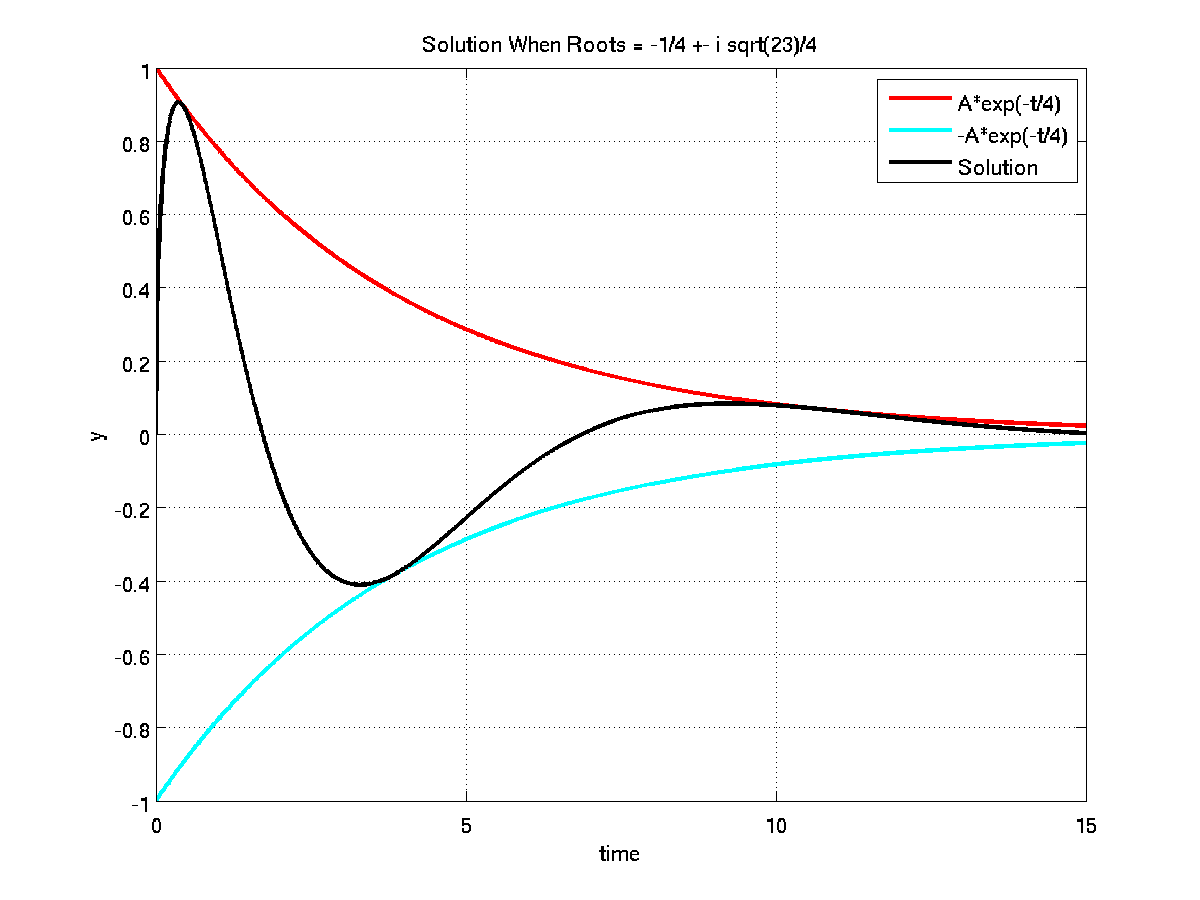
\includegraphics[height=12em]{img/decayOfConstantCoeffI}}
  
\end{frame}


\begin{frame}
  \frametitle{Example}

  \begin{eqnarray*}
    y'' + 6 y' + 13y & = & 0.
  \end{eqnarray*}

  \uncover<2->
  {
    \begin{eqnarray*}
      r^2 + 6r + 13 & = & 0, \\
      r & = & \frac{-6\pm\sqrt{36-52}}{2} \\
      & = & {\color{red}-3} \pm {\color{blue}2i} \\
      y & = & e^{{\color{red}-3t}} \lp A_1 \cos({\color{blue}2t}) + A_2 \sin({\color{blue}2t}) \rp.
    \end{eqnarray*}
  }

\end{frame}

\begin{frame}{Example - Continued}

    It decays like $e^{-3t}$ and oscillates with a period of $\pi$.

    \centerline{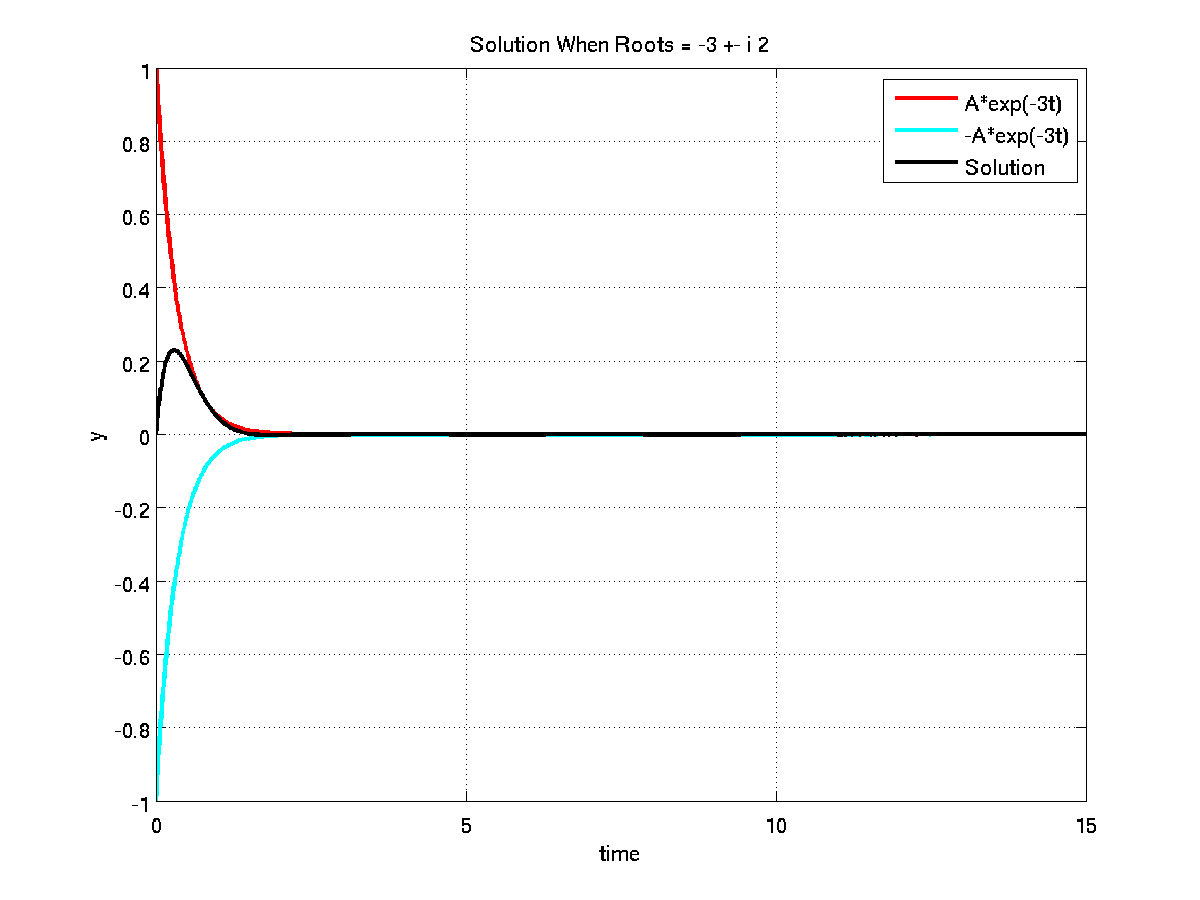
\includegraphics[height=12em]{img/decayOfConstantCoeffII}}
  
\end{frame}


\begin{frame}
  \frametitle{Example}

  \begin{eqnarray*}
    y^v - 4 y'& = & 0.
  \end{eqnarray*}

  \uncover<2->
  {
    \begin{eqnarray*}
      r^5 - 4r & = & 0, \\
      r & = & 0 \\
      \mathrm{or~} r^4 & = & 4 \\
      & = & \sqrt{2},~\sqrt{2}e^{i \pi/2}, ~ \sqrt{2}e^{i \pi},~ \sqrt{2}e^{i 3\pi/2} \\
      & = & \sqrt{2},~i\sqrt{2},~-\sqrt{2},~-i\sqrt{2} \\
      y & = & C_1 + C_2 e^{\sqrt{2}t} + C_3 e^{-\sqrt{2}t} +
      A_1 \cos(\sqrt{2}t) + A_2 \sin(\sqrt{2}t).
    \end{eqnarray*}
  }

  \uncover<3->
  {
    The dominant growth term is $e^{\sqrt{2}t}$. 
  }

\end{frame}

\subsection{An LRC Circuit}

\begin{frame}
  \frametitle{An LRC Circuit}

  An LRC circuit has a 30,0000 ohm resistor, a $5\times 10^{-6}$ F
  capacitor, and a 2000 Henries Inductor. Find the general equation
  describing  the charge in the capacitor at any time.

  \only<1>
  {
    % Graphic for TeX using PGF
% Title: /home/black/write/class/de/math232-12/ODE-Recitation-Activities/notes/img/LRCcircuit.dia
% Creator: Dia v0.97.2
% CreationDate: Wed Sep 18 10:33:40 2013
% For: black
% \usepackage{tikz}
% The following commands are not supported in PSTricks at present
% We define them conditionally, so when they are implemented,
% this pgf file will use them.
\ifx\du\undefined
  \newlength{\du}
\fi
\setlength{\du}{15\unitlength}
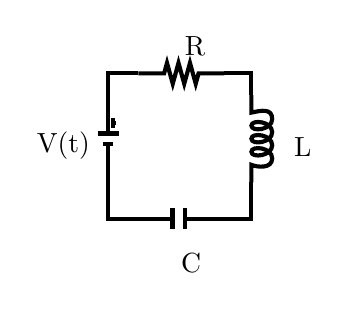
\begin{tikzpicture}
\pgftransformxscale{0.500000}
\pgftransformyscale{-0.500000}
\definecolor{dialinecolor}{rgb}{0.000000, 0.000000, 0.000000}
\pgfsetstrokecolor{dialinecolor}
\definecolor{dialinecolor}{rgb}{1.000000, 1.000000, 1.000000}
\pgfsetfillcolor{dialinecolor}
\pgfsetlinewidth{0.100000\du}
\pgfsetdash{}{0pt}
\pgfsetdash{}{0pt}
\pgfsetbuttcap
\pgfsetmiterjoin
\pgfsetlinewidth{0.100000\du}
\pgfsetbuttcap
\pgfsetmiterjoin
\pgfsetdash{}{0pt}
\definecolor{dialinecolor}{rgb}{0.000000, 0.000000, 0.000000}
\pgfsetstrokecolor{dialinecolor}
\draw (2.900000\du,9.550000\du)--(2.900000\du,10.800000\du);
\pgfsetbuttcap
\pgfsetmiterjoin
\pgfsetdash{}{0pt}
\definecolor{dialinecolor}{rgb}{0.000000, 0.000000, 0.000000}
\pgfsetstrokecolor{dialinecolor}
\draw (2.400000\du,10.800000\du)--(3.400000\du,10.800000\du);
\pgfsetbuttcap
\pgfsetmiterjoin
\pgfsetdash{}{0pt}
\definecolor{dialinecolor}{rgb}{0.000000, 0.000000, 0.000000}
\pgfsetstrokecolor{dialinecolor}
\draw (2.650000\du,11.300000\du)--(3.150000\du,11.300000\du);
\pgfsetbuttcap
\pgfsetmiterjoin
\pgfsetdash{}{0pt}
\definecolor{dialinecolor}{rgb}{0.000000, 0.000000, 0.000000}
\pgfsetstrokecolor{dialinecolor}
\draw (3.150000\du,10.050000\du)--(3.150000\du,10.550000\du);
\pgfsetbuttcap
\pgfsetmiterjoin
\pgfsetdash{}{0pt}
\definecolor{dialinecolor}{rgb}{0.000000, 0.000000, 0.000000}
\pgfsetstrokecolor{dialinecolor}
\draw (3.025000\du,10.300000\du)--(3.275000\du,10.300000\du);
\pgfsetbuttcap
\pgfsetmiterjoin
\pgfsetdash{}{0pt}
\definecolor{dialinecolor}{rgb}{0.000000, 0.000000, 0.000000}
\pgfsetstrokecolor{dialinecolor}
\draw (2.900000\du,11.300000\du)--(2.900000\du,12.550000\du);
\pgfsetlinewidth{0.100000\du}
\pgfsetdash{}{0pt}
\pgfsetdash{}{0pt}
\pgfsetbuttcap
\pgfsetmiterjoin
\pgfsetlinewidth{0.100000\du}
\pgfsetbuttcap
\pgfsetmiterjoin
\pgfsetdash{}{0pt}
\definecolor{dialinecolor}{rgb}{0.000000, 0.000000, 0.000000}
\pgfsetstrokecolor{dialinecolor}
\draw (4.350000\du,7.900000\du)--(5.595000\du,7.900000\du)--(5.733333\du,7.400000\du)--(6.010000\du,8.400000\du)--(6.286667\du,7.400000\du)--(6.563333\du,8.400000\du)--(6.840000\du,7.400000\du)--(7.116667\du,8.400000\du)--(7.255000\du,7.900000\du)--(8.500000\du,7.900000\du);
\pgfsetlinewidth{0.100000\du}
\pgfsetdash{}{0pt}
\pgfsetdash{}{0pt}
\pgfsetbuttcap
\pgfsetmiterjoin
\pgfsetlinewidth{0.100000\du}
\pgfsetbuttcap
\pgfsetmiterjoin
\pgfsetdash{}{0pt}
\definecolor{dialinecolor}{rgb}{0.000000, 0.000000, 0.000000}
\pgfsetstrokecolor{dialinecolor}
\pgfpathmoveto{\pgfpoint{9.800000\du}{8.950000\du}}
\pgfpathlineto{\pgfpoint{9.800000\du}{9.790000\du}}
\pgfpathcurveto{\pgfpoint{10.300000\du}{9.685000\du}}{\pgfpoint{10.800000\du}{9.580000\du}}{\pgfpoint{10.800000\du}{10.105000\du}}
\pgfpathcurveto{\pgfpoint{10.800000\du}{10.630000\du}}{\pgfpoint{9.800000\du}{10.735000\du}}{\pgfpoint{9.800000\du}{10.420000\du}}
\pgfpathcurveto{\pgfpoint{9.800000\du}{10.105000\du}}{\pgfpoint{10.800000\du}{10.210000\du}}{\pgfpoint{10.800000\du}{10.735000\du}}
\pgfpathcurveto{\pgfpoint{10.800000\du}{11.260000\du}}{\pgfpoint{9.800000\du}{11.365000\du}}{\pgfpoint{9.800000\du}{11.050000\du}}
\pgfpathcurveto{\pgfpoint{9.800000\du}{10.735000\du}}{\pgfpoint{10.800000\du}{10.840000\du}}{\pgfpoint{10.800000\du}{11.365000\du}}
\pgfpathcurveto{\pgfpoint{10.800000\du}{11.890000\du}}{\pgfpoint{9.800000\du}{11.995000\du}}{\pgfpoint{9.800000\du}{11.680000\du}}
\pgfpathcurveto{\pgfpoint{9.800000\du}{11.365000\du}}{\pgfpoint{10.800000\du}{11.470000\du}}{\pgfpoint{10.800000\du}{11.995000\du}}
\pgfpathcurveto{\pgfpoint{10.800000\du}{12.520000\du}}{\pgfpoint{10.050000\du}{12.415000\du}}{\pgfpoint{9.800000\du}{12.310000\du}}
\pgfpathlineto{\pgfpoint{9.800000\du}{13.150000\du}}
\pgfusepath{stroke}
\pgfsetlinewidth{0.100000\du}
\pgfsetdash{}{0pt}
\pgfsetdash{}{0pt}
\pgfsetbuttcap
\pgfsetmiterjoin
\pgfsetlinewidth{0.100000\du}
\pgfsetbuttcap
\pgfsetmiterjoin
\pgfsetdash{}{0pt}
\definecolor{dialinecolor}{rgb}{0.000000, 0.000000, 0.000000}
\pgfsetstrokecolor{dialinecolor}
\draw (4.800000\du,14.900000\du)--(6.000000\du,14.900000\du);
\pgfsetbuttcap
\pgfsetmiterjoin
\pgfsetdash{}{0pt}
\definecolor{dialinecolor}{rgb}{0.000000, 0.000000, 0.000000}
\pgfsetstrokecolor{dialinecolor}
\draw (6.000000\du,14.400000\du)--(6.000000\du,15.400000\du);
\pgfsetbuttcap
\pgfsetmiterjoin
\pgfsetdash{}{0pt}
\definecolor{dialinecolor}{rgb}{0.000000, 0.000000, 0.000000}
\pgfsetstrokecolor{dialinecolor}
\draw (6.600000\du,14.400000\du)--(6.600000\du,15.400000\du);
\pgfsetbuttcap
\pgfsetmiterjoin
\pgfsetdash{}{0pt}
\definecolor{dialinecolor}{rgb}{0.000000, 0.000000, 0.000000}
\pgfsetstrokecolor{dialinecolor}
\draw (6.600000\du,14.900000\du)--(7.800000\du,14.900000\du);
\pgfsetlinewidth{0.100000\du}
\pgfsetdash{}{0pt}
\pgfsetdash{}{0pt}
\pgfsetmiterjoin
\pgfsetbuttcap
{
\definecolor{dialinecolor}{rgb}{0.000000, 0.000000, 0.000000}
\pgfsetfillcolor{dialinecolor}
% was here!!!
{\pgfsetcornersarced{\pgfpoint{0.000000\du}{0.000000\du}}\definecolor{dialinecolor}{rgb}{0.000000, 0.000000, 0.000000}
\pgfsetstrokecolor{dialinecolor}
\draw (8.500000\du,7.900000\du)--(9.800000\du,7.900000\du)--(9.800000\du,8.950000\du);
}}
\pgfsetlinewidth{0.100000\du}
\pgfsetdash{}{0pt}
\pgfsetdash{}{0pt}
\pgfsetmiterjoin
\pgfsetbuttcap
{
\definecolor{dialinecolor}{rgb}{0.000000, 0.000000, 0.000000}
\pgfsetfillcolor{dialinecolor}
% was here!!!
{\pgfsetcornersarced{\pgfpoint{0.000000\du}{0.000000\du}}\definecolor{dialinecolor}{rgb}{0.000000, 0.000000, 0.000000}
\pgfsetstrokecolor{dialinecolor}
\draw (2.900000\du,9.550000\du)--(2.900000\du,7.900000\du)--(4.350000\du,7.900000\du);
}}
\pgfsetlinewidth{0.100000\du}
\pgfsetdash{}{0pt}
\pgfsetdash{}{0pt}
\pgfsetmiterjoin
\pgfsetbuttcap
{
\definecolor{dialinecolor}{rgb}{0.000000, 0.000000, 0.000000}
\pgfsetfillcolor{dialinecolor}
% was here!!!
{\pgfsetcornersarced{\pgfpoint{0.000000\du}{0.000000\du}}\definecolor{dialinecolor}{rgb}{0.000000, 0.000000, 0.000000}
\pgfsetstrokecolor{dialinecolor}
\draw (9.800000\du,13.150000\du)--(9.800000\du,13.150000\du)--(9.800000\du,14.900000\du)--(7.800000\du,14.900000\du);
}}
\pgfsetlinewidth{0.100000\du}
\pgfsetdash{}{0pt}
\pgfsetdash{}{0pt}
\pgfsetmiterjoin
\pgfsetbuttcap
{
\definecolor{dialinecolor}{rgb}{0.000000, 0.000000, 0.000000}
\pgfsetfillcolor{dialinecolor}
% was here!!!
{\pgfsetcornersarced{\pgfpoint{0.000000\du}{0.000000\du}}\definecolor{dialinecolor}{rgb}{0.000000, 0.000000, 0.000000}
\pgfsetstrokecolor{dialinecolor}
\draw (2.900000\du,12.550000\du)--(2.900000\du,14.900000\du)--(4.800000\du,14.900000\du);
}}
% setfont left to latex
\definecolor{dialinecolor}{rgb}{0.000000, 0.000000, 0.000000}
\pgfsetstrokecolor{dialinecolor}
\node[anchor=west] at (6.050000\du,6.600000\du){R};
% setfont left to latex
\definecolor{dialinecolor}{rgb}{0.000000, 0.000000, 0.000000}
\pgfsetstrokecolor{dialinecolor}
\node[anchor=west] at (5.865000\du,17.055000\du){C};
% setfont left to latex
\definecolor{dialinecolor}{rgb}{0.000000, 0.000000, 0.000000}
\pgfsetstrokecolor{dialinecolor}
\node[anchor=west] at (-1.080000\du,11.360000\du){V(t)};
% setfont left to latex
\definecolor{dialinecolor}{rgb}{0.000000, 0.000000, 0.000000}
\pgfsetstrokecolor{dialinecolor}
\node[anchor=west] at (7.450000\du,16.200000\du){};
% setfont left to latex
\definecolor{dialinecolor}{rgb}{0.000000, 0.000000, 0.000000}
\pgfsetstrokecolor{dialinecolor}
\node[anchor=west] at (11.315000\du,11.455000\du){L};
\end{tikzpicture}

  }

  \uncover<2->
  {
    \begin{eqnarray*}
      2000 Q'' + 30,000 Q' + \frac{Q}{5\times 10^{-6}} & = & 0 \\
      Q'' + 15 Q' + 100 Q & = & 0 \\
      r^2 + 15 r + 100 & = & 0
    \end{eqnarray*}
    \begin{eqnarray*}
      r & = & \frac{-15\pm\sqrt{15^2-400}}{2} \\
      r & = & \frac{-15}{2} \pm i\frac{5\sqrt{7}}{2} \\
      Q & = & e^{-15/2 t}
      \lp A_1 \cos\lp \frac{5\sqrt{7}}{2} t\rp + A_2 \sin\lp \frac{5\sqrt{7}}{2} t \rp \rp.
    \end{eqnarray*}

  }

\end{frame}

\subsection{Design a Spring Mass System}

\iftoggle{clicker}{%
\begin{frame}
  \frametitle{Clicker Quiz}

      \ifnum\value{clickerQuiz}=1{%

        \vfill

        What value of $\omega$ will result in a period of 4 in the function
        \begin{eqnarray*}
          f(t) & = & \cos(\omega t)?
        \end{eqnarray*}

        \vfill

        \begin{tabular}{ll}
          A: & $8\pi$ \\ [12pt]
          B: & $\frac{\pi}{2}$ \\  [12pt]
          C: & $\frac{1}{\pi}$ \\  [12pt]
          D: & $\frac{2}{\pi}$
        \end{tabular}

        \vfill

      }\fi

      \ifnum\value{clickerQuiz}=2{%

        \vfill

        What value of $\omega$ will result in a period of 3 in the function
        \begin{eqnarray*}
          f(t) & = & \cos(\omega t)?
        \end{eqnarray*}

        \vfill

        \begin{tabular}{ll}
          A: & $6\pi$ \\ [12pt]
          B: & $\frac{2\pi}{3}$ \\  [12pt]
          C: & $\frac{1}{2\pi}$ \\  [12pt]
          D: & $\frac{3}{2\pi}$
        \end{tabular}

        \vfill

     }\fi

     \ifnum\value{clickerQuiz}=3{%
       What value of $\omega$ will result in a period of 5 in the function
        \begin{eqnarray*}
          f(t) & = & \cos(\omega t)?
        \end{eqnarray*}

        \vfill

        \begin{tabular}{ll}
          A: & $10\pi$ \\ [12pt]
          B: & $\frac{2\pi}{5}$ \\  [12pt]
          C: & $\frac{1}{2\pi}$ \\  [12pt]
          D: & $\frac{5}{2\pi}$
        \end{tabular}

        \vfill

    }\fi


\end{frame}
}


\begin{frame}
  \frametitle{Design a Spring Mass System}

  Design a spring mass system so that a spring with spring constant
  $k=0.2$ N/m will oscillate a mass through two oscillations every
  three seconds, and the amplitude should decay like $e^{-t/2}$.

  \uncover<2->
  {
    \begin{eqnarray*}
      m x'' + bx' + 0.2x & = & 0. \\
      m r^2 + br + 0.2 & = & 0, \\
      r & = & \frac{-b\pm\sqrt{{\color{red}b^2-.8m}}}{2m}, \\
      r & = & \frac{-b}{2m} \pm {\color{fuchsia}i} \frac{\sqrt{{\color{red}.8m - b^2}}}{2m}.
    \end{eqnarray*}

  }

\end{frame}


\begin{frame}

  The solution satisfies the following equation
  \begin{eqnarray*}
    x & = & e^{{\color{red}-b/2m t}}
    \lp A_1 \cos\lp{\color{blue}\frac{\sqrt{.8m - b^2}}{2m}} t\rp + A_2 \sin\lp {\color{blue}\frac{\sqrt{.8m - b^2}}{2m} t }\rp \rp.
  \end{eqnarray*}

  First the exponential term should satisfy
  \begin{eqnarray*}
    {\color{red}-\frac{b}{2m} t} & {\color{red}=} & {\color{red}-\frac{t}{2}} \\
    \Rightarrow b & = & m.
  \end{eqnarray*}

  Second, the frequency should satisfy
  \begin{eqnarray*}
    {\color{blue}\frac{\sqrt{.8m - b^2}}{2m} \frac{3}{2}} & {\color{blue}=} & {\color{blue}2 \pi}.
  \end{eqnarray*}

\end{frame}


\begin{frame}

  If we let $b=m$ and solve for $m$ in the second equation we get
  \begin{eqnarray*}
    m & = & \frac{0.8}{1 + \frac{64 \pi^2}{9}}, \\
    b & = & \frac{0.8}{1 + \frac{64 \pi^2}{9}}.
  \end{eqnarray*}

\end{frame}


% LocalWords:  Clarkson pausesection hideothersubsections LRC Henries
